\def\QRCODE{MASTER_mispa_TUT.IMG.wavelets_pythonqrcode.png}
\def\QRPAGE{http://www.iptutorials.science/tree/master/MASTER_mispa/TUT.IMG.wavelets/python}
\pcorrectionsection{Python correction}

% \begin{tikzpicture}[remember picture,overlay]
%   \fill[orange] 
%   (current page header area.north west) 
%     rectangle
%   ([xshift=100pt,yshift=0pt]current page.east|-current page header area.south east);
% \end{tikzpicture}


\begin{python}
import numpy as np
from scipy import misc
import matplotlib.pyplot as plt
\end{python}

\subsection{1D signals}
Two functions are required: a function (\pinline{simpleWaveDec}) that loops over the different scales and calls the second function (\pinline{waveSingleDec}) that performs the single step wavelet decomposition. Notice that the Haar wavelet is defined here with integer values (see Fig.\ref{fig:wavelets:python:haar}), so that the mental computation can be done easily.

\begin{figure}[htbp]
 \centering\caption{Haar wavelets. From wikipedia, author Omegatron.}%
 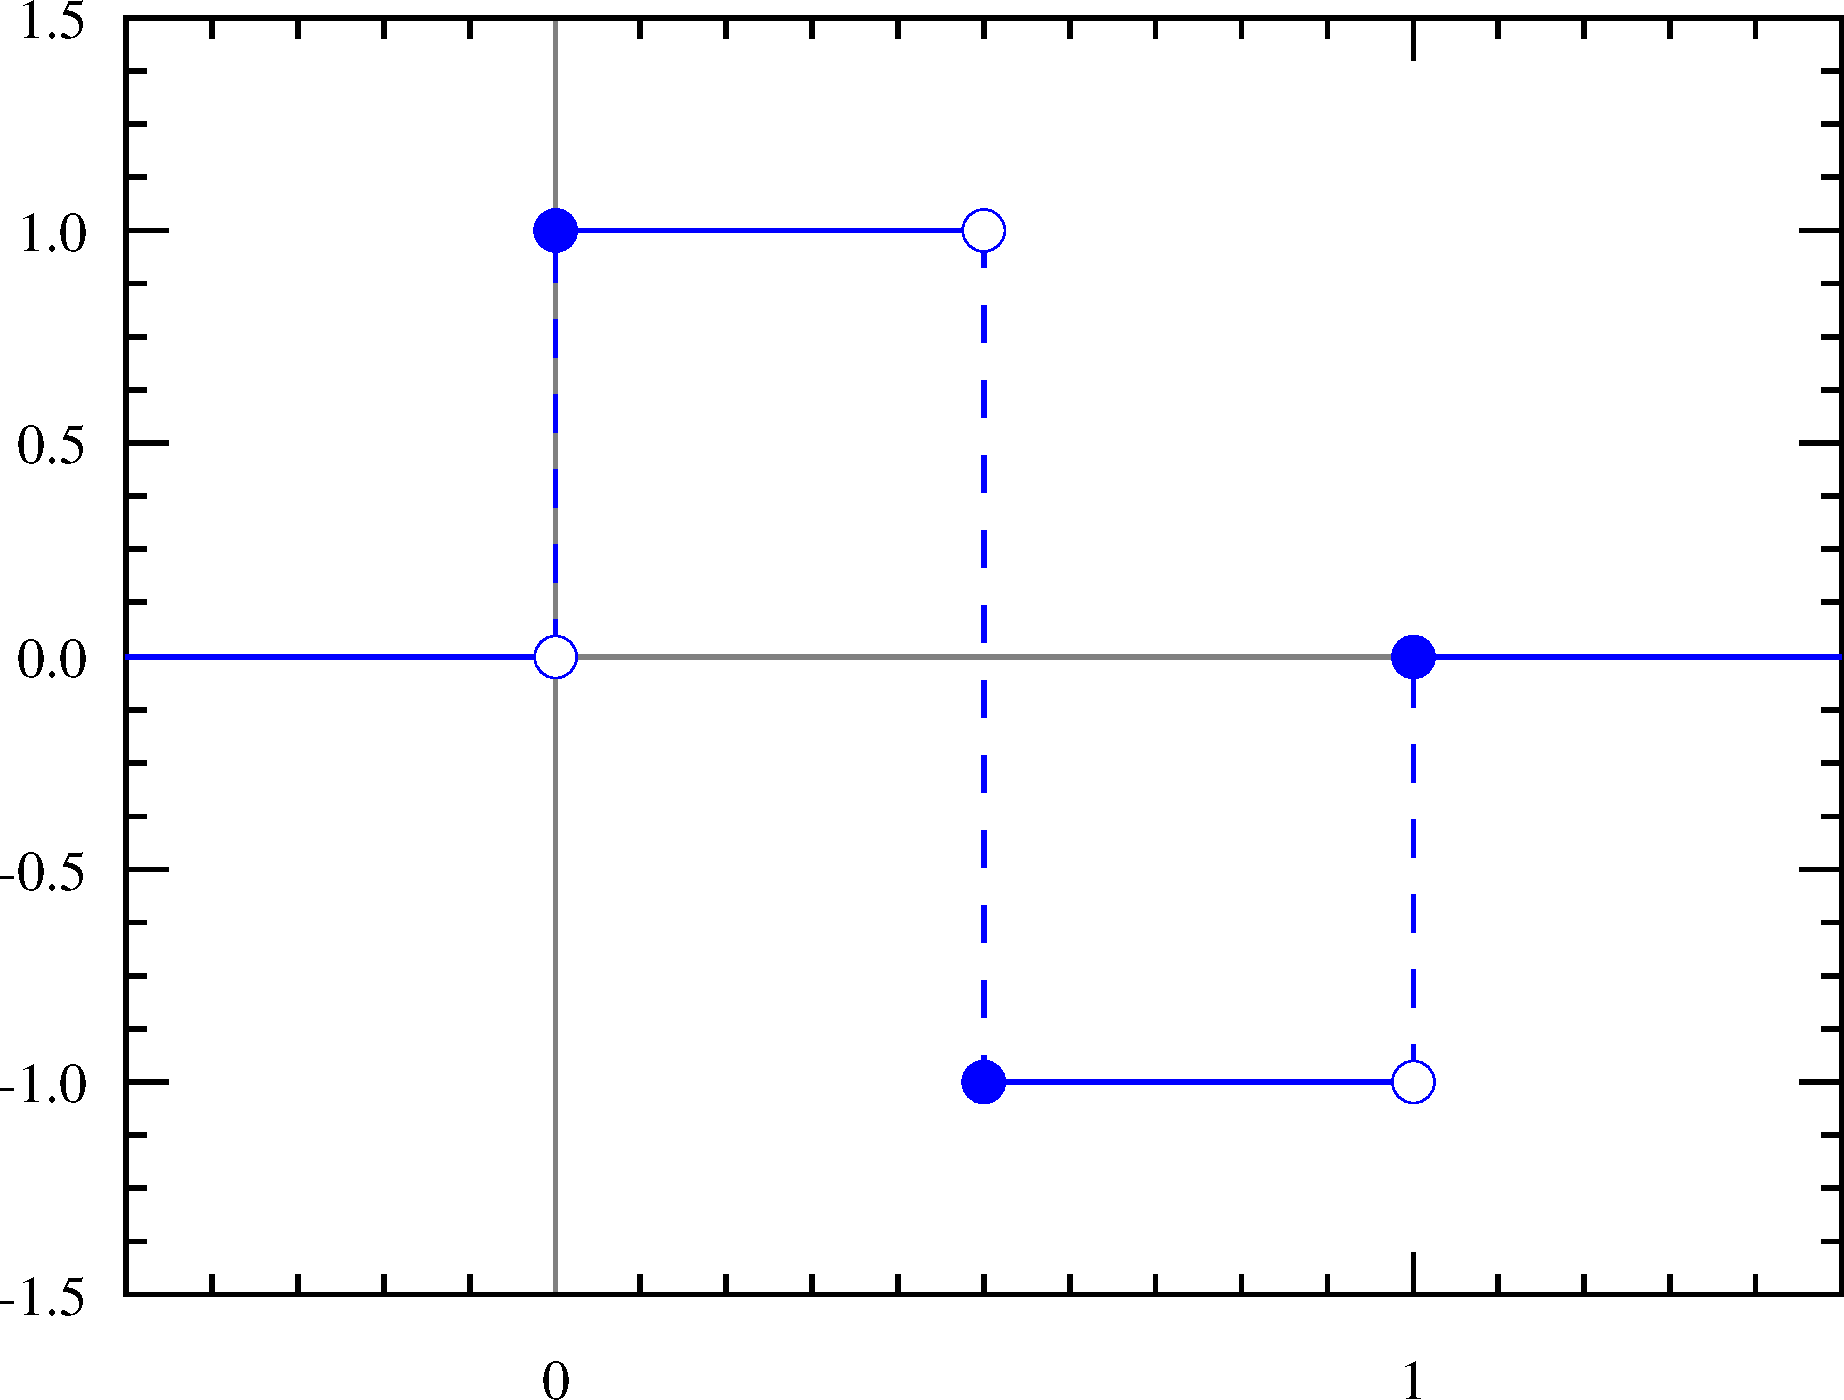
\includegraphics[width=.55\linewidth]{Haar_wavelet.pdf}%
 \label{fig:wavelets:python:haar}%
\end{figure}


\subsubsection{Simple 1D decomposition}
\begin{python}
def simpleWaveDec(signal, nb_scales):
    """
    wavelet decomposition of <signal> into <nb_scales> scales
    This function uses Haar wavelets for demonstration purposes.
    """
    # Haar Wavelets filters for decomposition and reconstruction
    ld = [1, 1];
    hd = [-1, 1];
    
    # transformation
    C=[];
    A = signal; # approximation
    for i in range(nb_scales):
        A, D = waveSingleDec(A, ld, hd);
        #get the coefficients
        C.append(D);
   
    C.append(A);
    return C;
\end{python}

\begin{python}
def waveSingleDec(signal, ld, hd):
    """
    1D wavelet decomposition into
    A: approximation vector
    D: detail vector
    ld: low pass filter
    hd: high pass filter
    """
    # convolution
    A = np.convolve(signal, ld, 'same');
    D = np.convolve(signal, hd, 'same');
    # subsampling
    A = A[1::2];
    D = D[1::2];
    return A, D;
\end{python}

\subsubsection{Simple 1D reconstruction}
The reconstruction starts from the highest scale and computes the approximation signal with the given details.
\begin{python}
def simpleWaveRec(C):
    """
    wavelet simple reconstruction function of a 1D signal
    C: Wavelet coefficients 
    The Haar wavelet is used
    """
    ld = np.array([1, 1]);
    hd = np.array([-1, 1]);
    lr = ld/2;
    hr = -hd/2;
    
    A = C[-1];
    for scale in reversed(C[:-2]):
        A = waveSingleRec(A, scale, lr, hr);
    return A;
\end{python}

\begin{python}
def waveSingleRec(a, d, lr, hr):
    """
    1D wavelet reconstruction at one scale
    a: vector of approximation
    d: vector of details
    lr: low pass filter defined by wavelet
    hr: high pass filter defined by wavelet
    This is Mallat algorithm.
    NB: to avoid side effects, the convolution function does not use the
    'same' option
    """
    approx = np.zeros((len(a)*2,));
    approx[::2] = a;
    approx = np.convolve(approx, lr);
    
    detail = np.zeros((len(a)*2,));
    detail[::2] = d;
    detail = np.convolve(detail, hr);
    # sum up approximation and details to reconstruct signal at lower scale
    approx = approx + detail;
    #get rid of last value
    approx = np.delete(approx, -1)
    return approx
\end{python}

\subsubsection{Results}
This is the result for the decomposition of the vector with 3 scales.
\begin{python}
s = [4, 8, 2, 3, 5, 18, 19, 20];
print(s)
C = simpleWaveDec(s, 3);
print(C)
srec = simpleWaveRec(C);
print(srec);
\end{python}

\begin{sh}
[4, 8, 2, 3, 5, 18, 19, 20]
[array([ -4,  -1, -13,  -1]), array([  7, -16]), array([-45]), array([79])]
\end{sh}


\subsection{2D signals}
\subsubsection{Decomposition}
The \pinline{simpleImageDec} function is the main interface. It takes the image as first parameter, and the number of scales of decomposition. It makes a call to \pinline{decWave2D} for the decomposition at one given scale. The latter uses the previous 1D decomposition method.

\begin{python}
def decWave2D(image, ld, hd):
    """
    % wavelet decomposition of a 2D image into four new images.
    % The image is supposed to be square, the size of it is a power of 2 in the
    % x and y dimensions.
    """

    # Decomposition on rows
    sx, sy = image.shape;

    LrA = np.zeros((sx, int(sy/2)));
    HrA = np.zeros((sx, int(sy/2)));
    
    for i in range(sx):
        A, D= waveSingleDec(image[i,:], ld, hd);
        LrA[i,:]= A;
        HrA[i,:]= D;

    # Decomposition on cols
    LcLrA = np.zeros((int(sx/2), int(sy/2)));
    HcLrA = np.zeros((int(sx/2), int(sy/2)));
    LcHrA = np.zeros((int(sx/2), int(sy/2)));
    HcHrA = np.zeros((int(sx/2), int(sy/2)));
    for j in range(int(sy/2)):
        A, D= waveSingleDec(LrA[:,j], ld, hd);
        LcLrA[:,j] = A;
        HcLrA[:,j] = D;
        
        A, D= waveSingleDec(HrA[:,j], ld, hd);
        LcHrA[:,j] = A;
        HcHrA[:,j] = D;
        
    return LcLrA, HcLrA, LcHrA, HcHrA
\end{python}

\begin{python}
def simpleImageDec(image, nb_scales):
    """
    wavelet decomposition of <image> into <nb_scales> scales
    This function uses Haar wavelets for demonstration purposes.
    """

    #Haar Wavelets filters for decomposition and reconstruction
    ld = [1,1];
    hd = [-1, 1];

    #transformation
    C=[];
    A = image; # first approximation

    coeffs = [];
    for i in range(nb_scales):
        [A, HcLrA, LcHrA, HcHrA] = decWave2D(A, ld, hd);
        coeffs.append( HcLrA);
        coeffs.append(LcHrA);
        coeffs.append(HcHrA);
        #set the coefficients
        C.append(coeffs.copy());
        coeffs.clear();
    C.append(A);
    return C;
\end{python}


\subsubsection{2D reconstruction}
The \pinline{simpleImageRec} function performs the reconstruction of a multiscale wavelet decomposition. The \pinline{recWave2D} performs the reconstruction of one scale.

\begin{python}
def recWave2D(LcLrA, HcLrA, LcHrA, HcHrA, lr, hr):
    """
    Reconstruction of an image from lr and hr filters and from the wavelet decomposition.
    A: resulting (reconstructed) image
    
    NB: This algorithm supposes that the number of pixels in x and y dimensions is a power of 2.
    """

    sx, sy = LcLrA.shape;
    
    # Allocate temporary matrices
    LrA = np.zeros((sx*2, sy));
    HrA = np.zeros((sx*2, sy));
    A   = np.zeros((sx*2, sy*2));
    
    #Reconstruct from cols
    for j in range(sy):
        LrA[:,j] = waveSingleRec(LcLrA[:,j], HcLrA[:,j], lr, hr);
        HrA[:,j] = waveSingleRec(LcHrA[:,j], HcHrA[:,j], lr, hr);
    
    # Reconstruct from rows
    for i in range(sx*2):
        A[i,:] = waveSingleRec(LrA[i,:], HrA[i,:], lr, hr);
        
    return A;
\end{python}

\begin{python}def simpleImageRec(C):
    """
    wavelet reconstruction of an image described by the wavelet coefficients C 
    """
    #The Haar wavelet is used
    ld = np.array([1, 1]);
    hd = np.array([-1, 1]);
    lr = ld/2;
    hr = -hd/2;
    A = C[-1];
    for scale in reversed(C[:-1]):
        A = recWave2D(A, scale[0], scale[1], scale[2], lr, hr);
        
    return A;
\end{python}

\subsubsection{Results}
The illustration Fig. \ref{fig:wavelets:python:lena_lvl} is obtained by the following code. The useful functions are presented below.
\begin{sh}
I = imageio.imread('lena256.png');
C = simpleImageDec(I, 3);
Irec = simpleImageRec(C);
plt.imshow(Irec);
plt.show()
\end{sh}

The image is recursively split into 4 areas, where the left upper corner is the approximation, and the three others are the details. As the details can have negative values, the intensities are adjusted in order to display the image correctly.
\begin{python}
def displayImageDec( C ):
    """
    Construct a single image from a wavelet decomposition
    C: the decomposition
    """
    n, m = C[0][0].shape;
    A = np.zeros((2*n, 2*m));
    prev = C[-1];
    for s, scales in reversedEnumerate(C[:-1]):
      
        ns = n / 2**(s-1);
        ms = m / 2**(s-1); 
        T = imdec2im(prev, scales);
        A[0:int(ns), 0:int(ms)] = T;
        prev = A[0:int(ns), 0:int(ms)];
    return prev
\end{python}

These two functions \pinline{adjust} and \pinline{reversedEnumerate} are used to simplify the notations. The first one performs a linear stretching of the image intensities, and the second one allows an enumeration of a list in a reverse order.
\begin{python}
def adjust(I):
    """
    simple image intensity stretching
    return I
    """
    I = I - np.min(I);
    I = I / np.max(I);
    return I;

def reversedEnumerate(l):
    """
    Utility function to perform reverse enumerate of a list
    returns zip
    """
    return zip(range(len(l)-1, -1, -1), l[::-1]);
\end{python}


\begin{python}
def imdec2im(LcLrA, lvlC):
    """
    constructs a single image from:
    LcLrA: the approximation image
    lvlC: the wavelet decomposition at one level
    
    for display purposes    
    """
    
    HcLrA=lvlC[0];
    LcHrA=lvlC[1];
    HcHrA=lvlC[2];
    n, m = HcLrA.shape;
    
    A = np.zeros((2*n, 2*m));
    
    # Approximation image can be with high values when using Haar coefficients
    A[0:n, 0:m] =adjust(LcLrA);
    
    # details are low, and can be negative
    A[0:n, m:2*m] = adjust(HcLrA);
    A[n:2*n, 0:m] = adjust(LcHrA,);
    A[n:2*n, m:2*m] = adjust(HcHrA);
    
    return A;
\end{python}

\begin{figure}[H]
 \centering\caption{(Haar) Wavelet decomposition of the Lena image.}%
 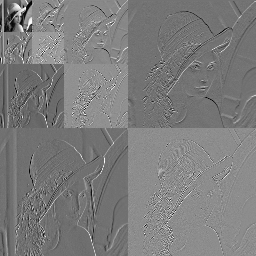
\includegraphics[width=.5\linewidth]{lena_wavelets_3.python.png}%
 \label{fig:wavelets:python:lena_lvl}%
\end{figure}


\subsection{Built-in functions}
An interesting module is \pinline{pywt}. This is illustrated by the following example. This gives the same results as previously, with the multiplication by $1/\sqrt{2}$.
\begin{python}
import pywt
cA, cD = pywt.dwt(s, 'haar');
print(cA, cD);
\end{python}

\begin{sh}
[ 8.48528137  3.53553391 16.26345597 27.57716447] 
[-2.82842712 -0.70710678 -9.19238816 -0.70710678]
\end{sh}

The continuous wavelet transform is applied in the following code and the result is displayed in Fig.\ref{fig:wavelets:python:cwt}.

\begin{python}
t = np.linspace(-1, 1, 1000, endpoint=False)
f1 =  3;
f2 = 50;
sig  = np.sin(2 * np.pi * f1 * t) + np.sin(2*np.pi * f2 * t);
widths = np.arange(1, 129)
coef, freqs=pywt.cwt(sig,widths,'morl')
fig = plt.figure();
plt.imshow(coef, extent=[-1, 1, 1, 31], cmap='PRGn', aspect='auto',
           vmax=abs(coef).max(), vmin=-abs(coef).max())  
plt.show() 
fig.savefig('cwt.python.pdf', bbox_inches='tight')
\end{python}

\begin{figure}[H]
 \centering\caption{Continuous wavelet decomposition of the sum of sinusoids.}%
 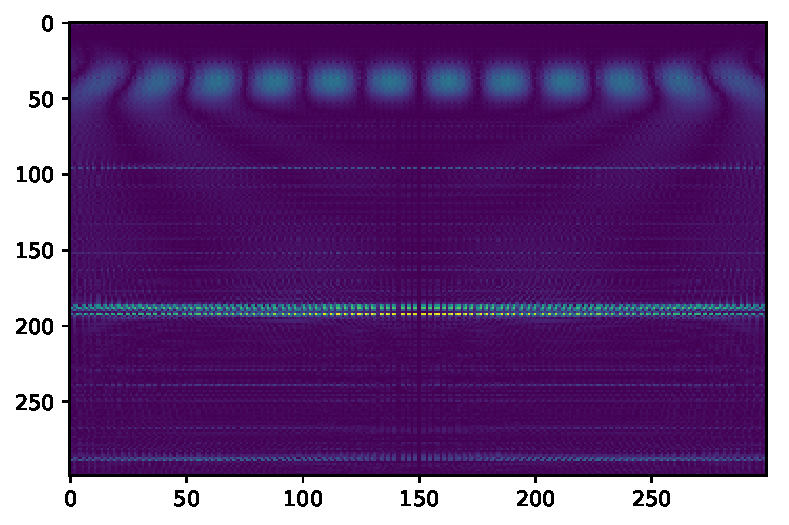
\includegraphics[width=.7\linewidth]{cwt.python.pdf}%
 \label{fig:wavelets:python:cwt}%
\end{figure}
